% USE PDFLatex!
% to correctly render Swedish characters

\documentclass{popsci}

\usepackage[utf8]{inputenc}
\usepackage[swedish, english]{babel}

\usepackage{fancyhdr}
\usepackage{titling}
\usepackage{color}
\usepackage{colortbl}
\usepackage{graphicx}
\usepackage{flushend}
\usepackage{lmodern}


% Please specify the presentation date
\presentationsdag{2023-06-16}

% use either of these commands to specify the title of your thesis
% \examensarbete{}
% To create a title in two rows, leave examensarbete blank and fill in examensarbeteTwoRows.
\examensarbeteTwoRows{Compression Algorithms for
Geometries Supporting Operations}

\students{Simon Erlandsson}{Leo Westerberg}
\supervisor{Hampus Londögård (AFRY AB), Jonas Skeppstedt (LTH)}
\examiner{Per Andersson (LTH)}

% Your pop-sci title should be different (more catchy) than your thesis title
\title{Hur kan stora kartor bli både snabba och små?}
%Hur kan stora kartor bli både snabba och små
%Hur gör man en stor karta liten och snabb

\begin{document}

% not more than 4 rows!
\theabstract{Komprimeringsalgoritmer används ofta för att minska storleken på kartdata. Problemet med konventionella metoder är att en stor mängd data måste packas upp vid minsta användning. Följaktligen undersöks hur stöd för effektiva operationer kan bibehållas efter komprimering utförts.}




{\noindent Dagens karttjänster består av en enorm mängd geometrisk data. Hus, stränder, länder och \mbox{vägar} kan alla representeras som polygoner och linjesegment. För att reducera storleken på geometrier används  komprimeringsalgoritmer för att ersätta redundant data, genom att \mbox{utnyttja} \mbox{statistiska} samband och mönster. \mbox{Problemet} med \mbox{konventionella} algoritmer är att de komprimerade \mbox{geometrierna} måste packas upp när de ska användas, oavsett vilken operation som ska \mbox{utföras}. Detta kan vara tidskrävande, i vissa fall så pass att \mbox{dekomprimeringen} i sig tar längre tid än själva \mbox{operationen}.

Detta examensarbetet har haft som syfte att undersöka om det finns en mellanväg - alltså ett sätt att få både snabba operationer och små geometrier. Arbetet mynnade ut i en implementation bestående av en kombination av befintliga komprimeringsalgoritmer, alternativa sätt att representera flyttalskoordinater och integrerat stöd för vissa geometriska operationer.

Implementationen nyttjar \emph{delta-kodning}, vilket innebär att istället för att spara varje koordinat till fullo, så sparas enbart mellanskillnaden. Denna är ofta mindre då geometrier används för att modulera världen. Tänk att för ett hus så är det rimligt att ange längden på väggarna, istället för varje hörns geografiska koordinat.

Delta-kodningen bildar en kedja av beroenden mellan koordinaterna, eftersom den tidigare \mbox{koordinaten} krävs för att avkoda värdet. Genom att bryta kedjan ibland, alltså spara hela koordinaten igen, så kan geometrier delas in i oberoende \emph{block}. 


\begin{figure}[!bth] % Use pictures in your pop-vet!
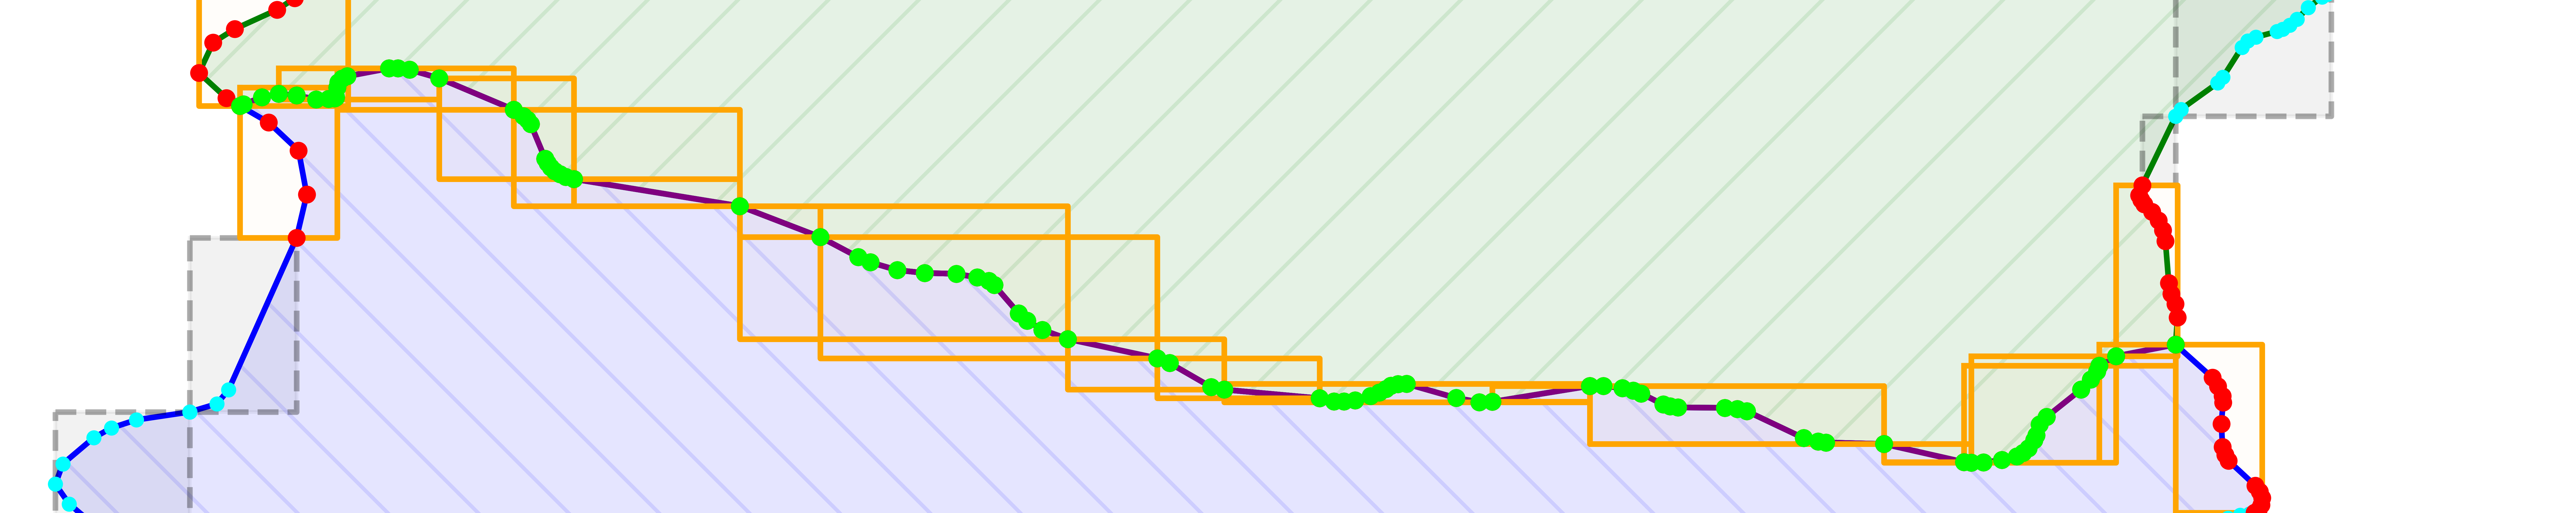
\includegraphics[width=\columnwidth]{images/popvet.png} 
%\caption{En fin bild}
\end{figure}
Genom att hoppa över de block som är irrelevanta så kan prestanda förbättras och tid sparas, eftersom enbart aktuella block dekomprimeras. Exempelvis, för att beräkna om två geometrier korsar varandra, så räcker det att undersöka de block vars ytor \mbox{överlappar} mellan geometrierna. 

Vid testning konstaterades att implementationen reducerade storleken med en faktor 2.56, jämfört med WKB och var 3.6 gånger snabbare än \mbox{referensimplementationen} som saknar optimerade operationer, vid beräkningen av \emph{snittet} över stora geometrier. Partiell dekomprimering av geometrier är till stor del outforskat inom akademin, men slutsatsen av arbetet är att området definitivt kan vara intressant att undersöka vidare.



}

\end{document}
